\section{Training an \ac{RNN} for \ac{ASR}}\label{ds}
As stated above, the focus for this project is not on training a state of the art \ac{STT} engine. Because the \ac{SW} algorithm used for local alignment is tolerant to a certain amount of errors in the transcripts, the \ac{RNN} need only be \textit{good enough} for the task at hand (\ac{FA}). If such a network can be trained under the given circumstances it could be used for any language in the \ac{ASR} stage of the pipeline. 

\subsection{Related research}

Hier etwas über Transfer Learning (z.B. wie in https://arxiv.org/pdf/1706.00290.pdf) und warum es nicht eingesetzt wurde (CNN anstatt RNN, Zeitaufwand). Layer Freezen bringt ausserdem offenbar auch nix. \parencite{budget}

\subsection{\textit{DeepSpeech}: A reference model}

A \ac{NN} that had quite an impact on \ac{ASR} was \textit{DeepSpeech} \parencite{deepspeech} which reached recognition rates near-par to human performance, despite using a comparably simpler than traditional speech systems. Because the relation between audio signal and text was learned \ac{E2E} the network was also pretty robust to distortions like background noise or speaker variation. An open source implementation of a \textit{DeepSpeech} model is available from Mozilla \footnote{\url{https://github.com/mozilla/DeepSpeech}}. This implementation uses a variant of of the \ac{RNN} originally proposed in the DeepSpeech paper \parencite{ctc_paper}\footnote{the variant used \ac{MFCC} as features whereas the original paper proposed raw spectrograms}. Since the implementation also uses a \ac{LM}, the quality of the model is measured as the percentage of misspelled or wrong words (referred to as \ac{WER}) or as the edit distance (also called Levenshtein distance or \ac{LER}). A pre-trained model for inference of English transcript can be downloaded, which achieves a \ac{WER} of just 6.5\%, which is close to what a human is able to recognize \parencite{mozillajourney} and serves as a reference model in this project.

\subsection{Exploiting the \textit{DeepSpeech} model}

Since the goal of this project is to provide alignments for any language, one possible approach would be to train a model using the existing Mozilla implementation by providing training-, validation- and test-data for each language. However, this approach has several drawbacks:

\begin{enumerate}
	\item The \textit{DeepSpeech} implementation was explicitly designed for \ac{ASR}. In such settings a low \ac{WER} is desirable. But because accurate speech recognition is not the main concern in this project, the architecture of the Mozilla implementation might be overly complicated. 
	\item The problem with above point is that more complex models usually require more training data. However, as for any neural network, the limiting factor for training a \ac{RNN} is often the lack of enough high quality training data. This becomes especially important when recordings in a minority language should be aligned. 
	\item The Mozilla implementation requires an (optional) \ac{LM}, which is tightly integrated with the training process which might not be available for the target languages.
\end{enumerate}

For these reasons, the architecture of the \ac{RNN} model from Mozilla was used only as a basis for a simplified version. This version should (hopefully) require less training data to converge and still produce partial transcriptions that can be aligned.

\subsection{A simpler model}

The implementation of the \ac{RNN} used for \ac{STT} in the previous IP8 project was done in Python using Keras\footnote{\url{https://keras.io}}. This model is further referred to as \textit{previous model}. Unfortunately, the previous model did not perform very well, i.e. it was not able to learn how to infer a transcript from a given sequence of feature vectors from a spectrogram. Furthermore, performance was a big issue, even though the \ac{RNN} was rather simple and no \ac{LM} was used. Training on aligned speech segments from the \textit{LibriSpeech} corpus would have taken approximately two months on a single \ac{GPU}. This duration is at consistent with the experience made by the Machine Learning team at Mozilla Research, which used a cluster of 16 \acsp{GPU} that required about a week \parencite{mozillajourney} to train a variant. For the purpose of this project however, such a long training time was a serious impediment.

In the course of this project, the previous model was examined more closely to find out what works best and to help the model converge. A few changes were made to arrive at a new model which was able to learn something meaningful. This model is further referred to as \textit{new model}. The new model started to infer transcripts that -- although still not perfect -- resembled the ground truth. The following list summarizes the differences between the previous and the new model:

\begin{itemize}
	\item \textbf{Optimizer}: The new model uses \ac{SGD} instead of Adam. Adam was used in the previous model because it is the Optimizer used in the Mozilla implementation of \ac{DS}. However, this optimizer did not seem to work for the simplified model.
	\item \textbf{number of features}: While the use of \ac{MFCC} as features was examined in the previous model, the number of features was set to $13$, a value which is found often used in acoustic modelling. The Mozilla implementation of \textit{DeepSpeech} however doubled this number to $26$. This is also the number of features used in the new model. Despite the increase in the number of features, this value is still much smaller than the $160$ filter banks used in the original \textit{DeepSpeech} model. The amount of training data is therefore still expected to be smaller than in the original model.
\end{itemize}

The new model constitutes a simplified variant of the original \textit{DeepSpeech} model with the following simplifications and changes applied:

\begin{itemize}
	\item \textbf{Different application of LM}: In the Mozilla implementation the use of a \ac{LM} is baked in with the training process, i.e. it is integrated in the decoding process. With The edit distance between prediction and ground truth is then included in the loss which is minimized. The simplified model also uses a \ac{LM}, but does not include it in the training process. Instead, the \ac{LM} is applied in some sort of post-processing to improve the quality of the decoded predictions.
	\item \textbf{Different features}: MFCC with 26 filter banks instead of Spectrogram with 161 filterbanks, because that's what the Mozilla implementation uses
	\item \textbf{No convolution in first layer}: Whereas \cite{ctc_paper} propose a convolution over time in the first layer for performance reasons, this is not done in the simplified model.
	\item \textbf{LSTM instead of SimpleRNN}: Whereas \cite{ctc_paper} deliberately refrain from using \ac{LSTM} cells for various reasons, the Mozilla implementation has shown that it is possible to implement the \textit{DeepSpeech} model using \ac{LSTM} cells. Since the simplified model is based on the Mozilla implementation, it also uses \ac{LSTM} cells.
	\item \textbf{dynamic alphabet}: The Mozilla implementation uses an alphabet with 29 characters\footnote{${a,b,c,...,z, space, apostrophe, blank}$}, which is also what is proposed in the \textit{DeepSpeech} paper. This is due to the fact that apostrophes are frequently found in English word tokens (like \textit{"don't"} or \textit{"isn't"}). The apostrophe is therefore an integral part of English words, but not for other languages. Vice versa, other languages may use a different alphabet (like German, where umlauts are prevalent). Because the number of characters in the alphabet determines the number of nodes in the output layer, the output layer has different shapes for different languages.
	\item \textbf{no context}: The \textit{DeepSpech} paper proposes using combining each feature vector $x_t$ (a frame in the spectrogram) with $C \in \left\{ 5,7,9 \right\}$ context frames. This context frame was dropped to keep the nuber of features in the input layer small. As a result, the first layer in the model only depends on the $26$ features of the feature vector $x_t$.
	\item \textbf{no convolution in input layer}: The \textit{DeepSpeech} paper proposes a series of optimization to reduce computational cost. Among these optimization is a convolution over time in the input layer with by striding with step size $2$. Because the context frame was dropped in this project, the striding was also not applied in order not to lose the information from the intermediate frames.
\end{itemize}


Figure \ref{model_architecture} shows the architecture proposed in the \textit{DeepSpeech} with the changes applied for this project. It looks similar to the one shown in the paper. Note the missing context frame, the use of \ac{MFCC} features and \ac{LSTM} cells in the recurrent layer.

\begin{figure}[h!]
	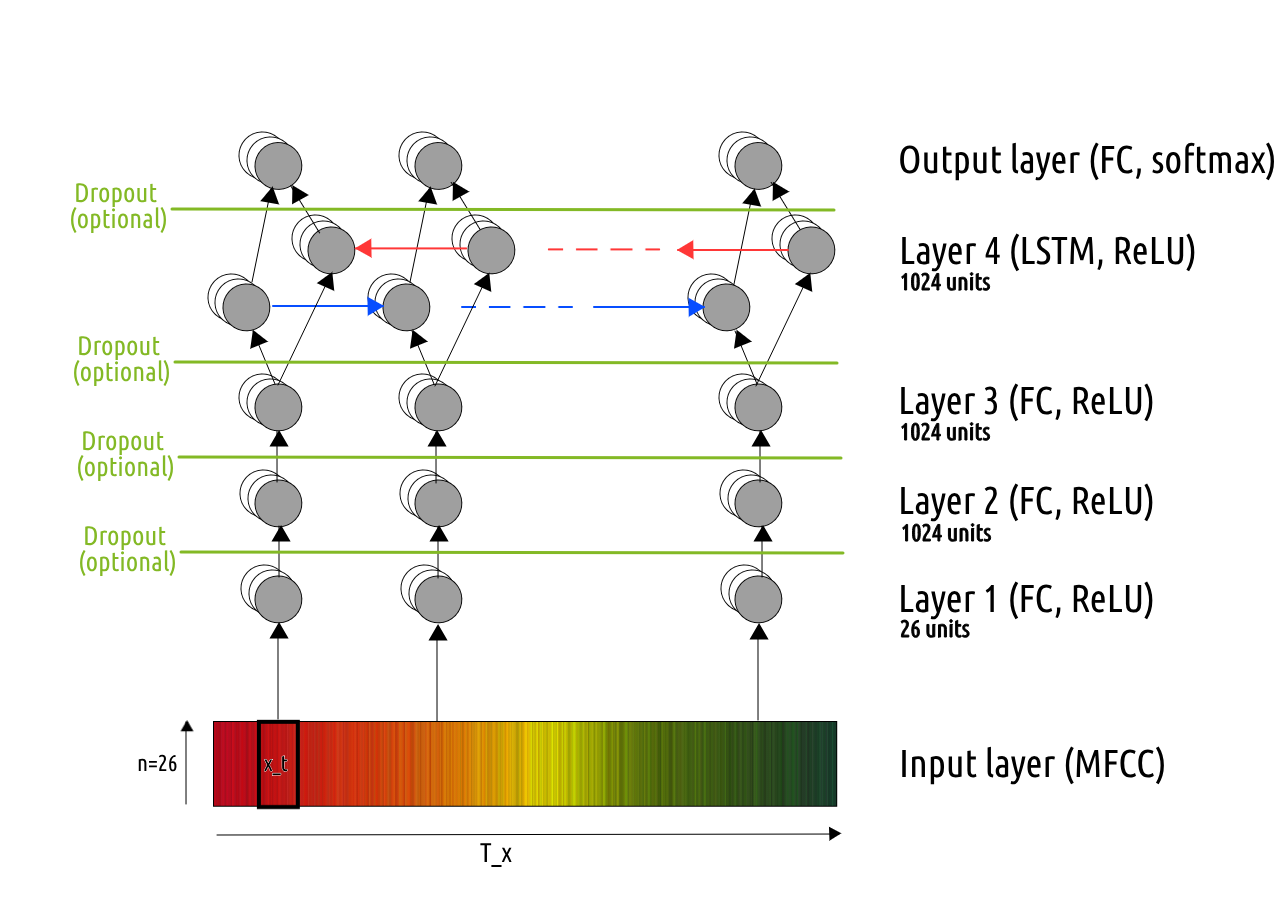
\includegraphics[width=\linewidth]{./img/model_architecture.png}
	\caption{Architecture of the simplified model. The cell type and the activation function is indicated in brackets for each layer (FC=Fully-Connected)}
	\label{model_architecture}
\end{figure}